\fvisa{Auld Lang Syne}{Should auld acquaintance be forgot}
{\footnotesize\textit{Melodi: Skotskt Traditionell}}\par
\vspace{10pt}
Should auld acquaintance be forgot,\\
and never brought to mind?\\
Should auld acquaintance be forgot,\\
and auld lang syne?\par
\vspace{10pt}
For auld lang syne, my jo,\\
for auld lang syne,\\
we'll tak' a cup o' kindness yet,\\
for auld lang syne.\par
\vspace{10pt}
And surely ye'll be your pint-stoup!\\
and surely I'll be mine!\\
And we'll tak' a cup o' kindness yet,\\
for auld lang syne.\par
\vspace{10pt}
For auld lang syne, my jo...\par
\vspace{10pt}
We twa hae run about the braes,\\
and pou'd the gowans fine;\\
But we've wander'd mony a weary fit,\\
sin' auld lang syne.\par
\vspace{10pt}
For auld lang syne, my jo...\par
\vspace{10pt}
We twa hae paidl'd in the burn,\\
frae morning sun till dine;\\
But seas between us braid hae roar'd\\
sin' auld lang syne.\par
\newpage
For auld lang syne, my jo...\par
\vspace{10pt}
And there's a hand, my trusty fiere!\\
and gie's a hand o' thine!\\
And we'll tak' a right gude-willie waught,\\
for auld lang syne.\par
\vspace{10pt}
For auld lang syne, my jo...\par
\vspace{15pt}
{\footnotesize\textit{``Scots pronunciation guide'' finnes på nästa uppslag. $\rightarrow$}}\par
\vfill
\index{ÃTasks@\uppercase{Tasks}}
\begin{center}
  \tiny{Tasks}\par
  \vspace{5pt}
  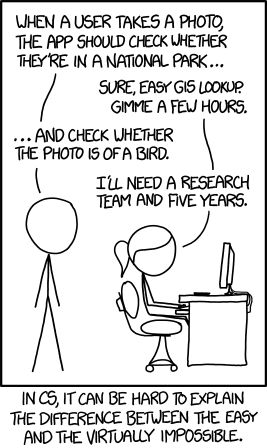
\includegraphics[keepaspectratio,width=0.45\textwidth]{elements/images/tasks.png}\par
  \vspace{5pt}
  \tiny{BY-NC 2.5 xkcd.com\\ In the 60s, Marvin Minsky assigned a couple of undergrads to spend the summer programming a computer to use a camera to identify objects in a scene. He figured they'd have the problem solved by the end of the summer. Half a century later, we're still working on it.}
\end{center}
\par
\vfill
\newpage
\svisa{Auld Lang Syne - Scots pronunciation guide}{Shid ald akwentans bee firgot}{Auld Lang Syne - \\Scots pronunciation guide}
{\footnotesize\textit{Melodi: Skotskt Traditionell}}\par
\vspace{10pt}
Shid ald akwentans bee firgot,\\
an nivir brocht ti mynd?\\
Shid ald akwentans bee firgot,\\
an ald lang syn?\par
\vspace{9pt}
Fir ald lang syn, ma jo,\\
fir ald lang syn,\\
wil tak a cup o kyndnes yet,\\
fir ald lang syn.\par
\vspace{9pt}
An sheerly yil bee yur pynt-staup!\\
an sheerly al bee myn!\\
An will tak a cup o kyndnes yet,\\
fir ald lang syn.\par
\vspace{9pt}
Fir ald lang syn, ma jo...\par
\vspace{9pt}
We twa hay rin aboot the braes,\\
an pood the gowans fyn;\\
Bit weev wandert monae a weery fet,\\
sin ald lang syn.\par
\vspace{9pt}
Fir ald lang syn, ma jo...\par
\vspace{9pt}
We twa hay pedilt in the burn,\\
fray mornin sun til dyn;\\
But seas between us bred hay roard\\
sin ald lang syn.\par
\newpage
Fir ald lang syn, ma jo...\par
\vspace{10pt}
An thers a han, my trustee feer!\\
an gees a han o thyn!\\
And we'll tak a richt gude-willie-waucht,\\
fir ald lang syn.\par
\vspace{10pt}
Fir ald lang syn, ma jo...
